\hypertarget{include_2thread__mpi_8h}{\section{include/thread\-\_\-mpi.h \-File \-Reference}
\label{include_2thread__mpi_8h}\index{include/thread\-\_\-mpi.\-h@{include/thread\-\_\-mpi.\-h}}
}


\-Convenience header file for non-\/\-M\-P\-I compatibility.  


{\ttfamily \#include \char`\"{}thread\-\_\-mpi/atomic.\-h\char`\"{}}\*
{\ttfamily \#include \char`\"{}thread\-\_\-mpi/threads.\-h\char`\"{}}\*
{\ttfamily \#include \char`\"{}thread\-\_\-mpi/numa\-\_\-malloc.\-h\char`\"{}}\*
{\ttfamily \#include \char`\"{}thread\-\_\-mpi/barrier.\-h\char`\"{}}\*
{\ttfamily \#include \char`\"{}thread\-\_\-mpi/event.\-h\char`\"{}}\*
{\ttfamily \#include \char`\"{}thread\-\_\-mpi/lock.\-h\char`\"{}}\*
{\ttfamily \#include \char`\"{}thread\-\_\-mpi/tmpi.\-h\char`\"{}}\*
{\ttfamily \#include \char`\"{}thread\-\_\-mpi/collective.\-h\char`\"{}}\*
\-Include dependency graph for thread\-\_\-mpi.\-h\-:
\nopagebreak
\begin{figure}[H]
\begin{center}
\leavevmode
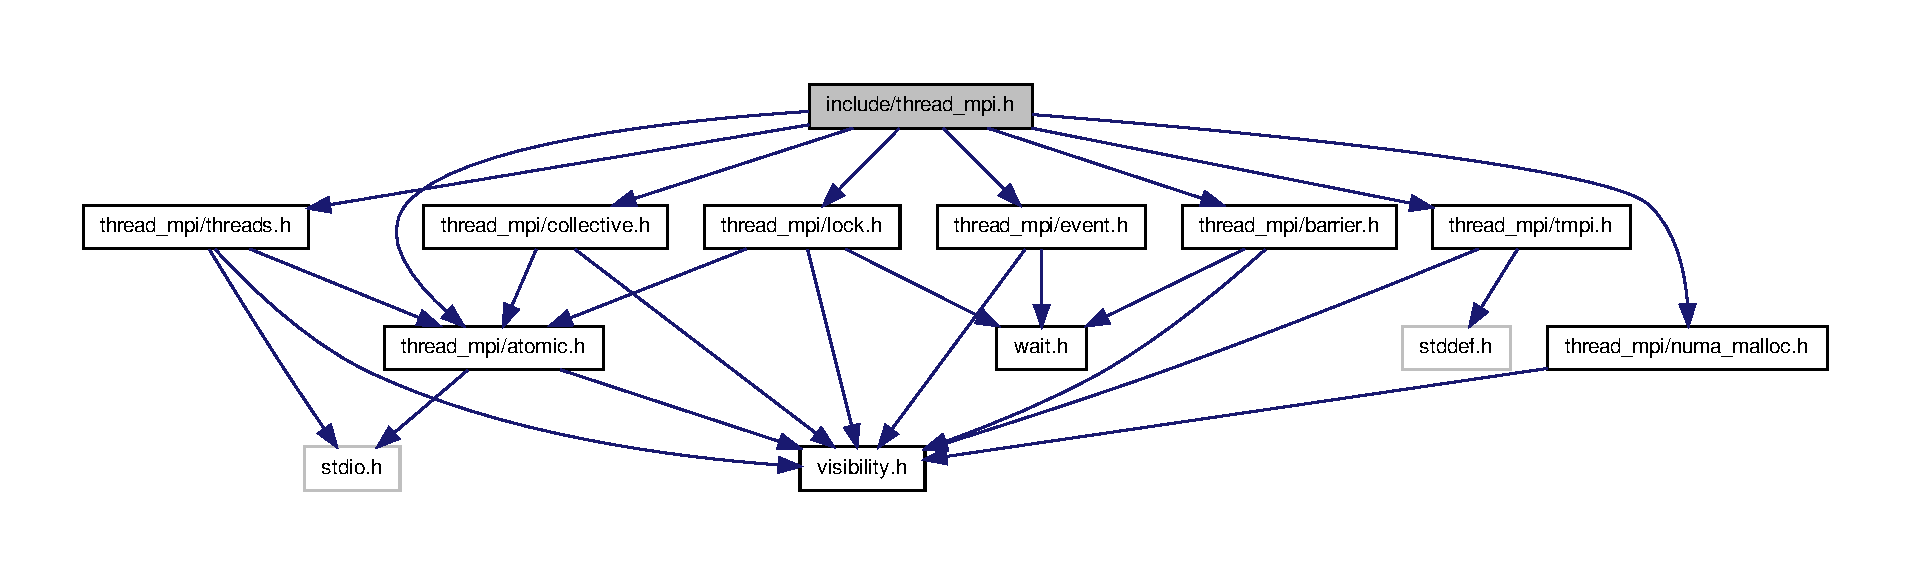
\includegraphics[width=350pt]{include_2thread__mpi_8h__incl}
\end{center}
\end{figure}


\subsection{\-Detailed \-Description}
\-Convenience header file for non-\/\-M\-P\-I compatibility. \-This file includes the t\-M\-P\-I header file thread\-\_\-mpi/tmpi.\-h, as well as thread\-\_\-mpi/threads.\-h and thread\-\_\-mpi/atomic.\-h header files. \-If you'd like to use the components individually, include the relevant header files directly. 